% !TEX root = ./final_report.tex
\section{Equations of Motion \label{sec:eom}}
The non-linear dynamic model of a quadcopter used in our project is that derived by Bouabdallah \cite{bouabdallah2007design}. The state of the system is

\begin{equation}
X = \left[\phi \; \dot{\phi} \; \theta \; \dot{\theta} \; \psi \; \dot{\psi} \; z \; \dot{z} \; x \; \dot{x} \; y \; \dot{y}
\right]^T
\end{equation}

and its dynamics are

\begin{equation}\label{eq:eom}
\frac{d X}{d t} = \left(
\begin{tabular}{c}
$\dot{\phi}$\\
$\dot{\theta}\dot{\psi}a_1 + \dot{\theta}a_2 U_4 + b_1 U_2$\\
$\dot{\theta}$\\
$\dot{\phi}\dot{\psi}a_3 - \dot{\phi}a_4 U_4 + b_2 U_3$\\
$\dot{\psi}$\\
$\dot{\theta}\dot{\phi}a_5 + b_3 U_4$\\
$\dot{z}$\\
$g - (\cos{\phi}\cos{\theta})\frac{1}{m}U_1$\\
$\dot{x}$\\
$(\cos{\phi}\sin{\theta}\cos{\psi} + \sin{\phi}\sin{\psi})\frac{1}{m}U_1$\\
$\dot{y}$\\
$(\cos{\phi}\sin{\theta}\sin{\psi} - \sin{\phi}\cos{\psi})\frac{1}{m}U_1$
\end{tabular}
\right) \;\; 
\end{equation}

where $a_1, a_2, a_3, a_4, a_5, b_1, b_2, b_3, m$ are constants related to physical properties of the quadcopter like moments of inertia and mass; $g$ is the acceleration due to gravity; $U_1$ is throttle control, $U_2$ is roll control, $U_3$ is pitch control, and $U_4$ is yaw control. The elements of the state vector are understood by observing Figure \ref{fig:coord_system}

\begin{figure}[h]
\centering
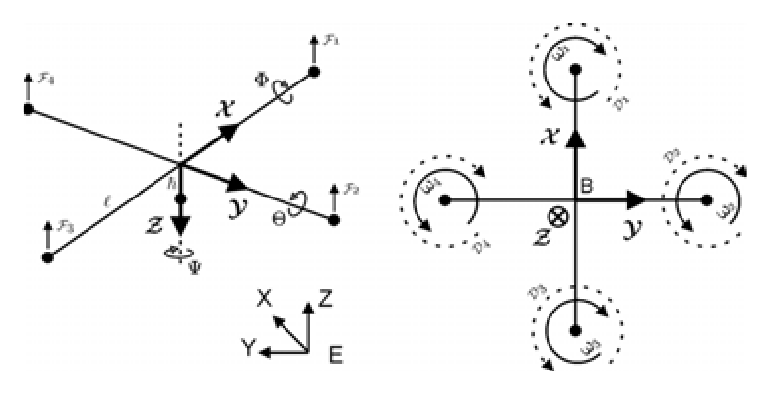
\includegraphics[width=8cm]{coordinate_system.png}
\caption{Quadcopter coordinate system  \cite{bouabdallah2007design}}
\label{fig:coord_system}
\end{figure}
%\centering
%\includegraphics[width=8cm]{2ndDeriv.eps}
%\caption{Comparison of $2^{\text{nd}}$ derivative values from smoothed data and the NN predictions}
%\label{fig:figure6}
%\end{figure}

%\newpage
%\begin{figure}[t]
%\centering
%\includegraphics[width=8cm]{SmoothPriceTrendPred.eps}
%\caption{Local optima recognition using the derivatives of the smoothed data}
%\label{fig:figure4}
%\end{figure}

\subsection{Linearization}
To design a controller for the quadcopter using tools for linear dynamics it is necessary to have an appropriate linearization of the equations of motion. We would like to find matrices $A$, $B$, and $G$ such that

\begin{equation}
\frac{d X}{d t} = A X + B U + G
\end{equation}
where $U$ is the control input vector $U = \left[U_1\; U_2\; U_3\; U_4\right]^T$. 

 By observing Equation \eqref{eq:eom}, we note that attempting a crude linearization about any given state could yield equations in which yaw, pitch, and roll controls are decoupled from displacements in space. This would lead to the problem of having to have an attitude controller wrapped by a spacial displacement controller. 
 
 Given that in this project we aim to explore the ability of MPC to handle complex systems, we choose to linearize the equations so the non-linear coupling between control inputs and state is taken into account. To this end, we add the control input vector to our state vector, and control the system via a change in the control inputs. By doing this, the state vector becomes
 
 \begin{equation}
 X = \left[\phi \; \dot{\phi} \; \theta \; \dot{\theta} \; \psi \; \dot{\psi} \; z \; \dot{z} \; x \; \dot{x} \; y \; \dot{y}\; U_1\; U_2\; U_3\; U_4
 \right]^T
 \end{equation}
 
 and the linearized equations of motion become
\begin{equation} \label{eq:lin_eom}
\frac{d X}{d t} = \left(
\begin{tabular}{c c c c c c c c c c c c}
$\hat{A}$ & $\hat{B}$ \\
${\bf 0}$ & ${\bf 0}$
\end{tabular}
\right)X +  
\left(
\begin{tabular}{c c c c c c c c c c c c}
$\hat{B}$ \\
${\bf 1}$
\end{tabular}
\right)\delta U + 
\left(
\begin{tabular}{c}
$\hat{G}$\\
${\bf 0}$
\end{tabular}\right)\;\; 
\end{equation}
where $\hat{A}$ and $\hat{B}$ linearize the coupling between state variables and controls, and $\delta U = \l[ \delta U_1 \;\delta U_2 \;\delta U_3 \;\delta U_4 \r]^T$ are the new control inputs. $\hat{G}$ contains constants coming from the coupled linearization.

To illustrate the procedure of finding the entries of matrices $\hat{A}, \hat{B}$, and $\hat{G}$, let us linearize the equation related to displacements in $z$ (altitude). From the non-linear Equation in \eqref{eq:eom}, we have
\begin{equation}\label{eq:z_eq}
\ddot{z} = g - ( \cos\phi \cos\theta)\frac{1}{m}U_1
\end{equation}

We can linearize $\cos \alpha$ about some angle $\alpha_0$ by setting 
\begin{equation}
\cos \alpha \approx \cos \alpha_0 + (\alpha - \alpha_0)(-\sin\alpha_0)
\end{equation}

With this in mind, \eqref{eq:z_eq} can be linearized about point $(\phi_0,\theta_0,U_{10})$ as
\begin{equation}\label{eq:lin_z_eq}
\begin{split}
\ddot{z} = g - \frac{1}{m}\bigg(&\frac{1}{3}U_1 \cos\phi \cos\theta \\
+ &\frac{1}{3}U_1 \cos\phi \cos\theta\\
 + &\frac{1}{3}U_1 \cos\phi \cos\theta\bigg)\\
 \approx g - \frac{1}{m}\bigg(& \frac{1}{3}U_1 \cos\phi_0 \cos\theta_0 \\
 + & \frac{1}{3}U_{10} \l[\cos \phi_0 + (\phi - \phi_0)(-\sin\phi_0)\r] \cos\theta_0 \\
+ & \frac{1}{3}U_{10} \cos\phi_0 \l[\cos \theta_0 + (\theta - \theta_0)(-\sin\theta_0)\r]\bigg)\\
\end{split}
\end{equation}
Note that in Equation \eqref{eq:lin_z_eq}, each state variable $\phi,\theta,U_1$ appears once and multiplies constants. Entries in $\hat{B}$ correspond to constants multiplying the control state variables $U$, entries in $\hat{A}$ correspond to constants multiplying attitude and displacement state variables, and entries in $\hat{G}$ correspond to the constants not multiplying a variable.
